% Options for packages loaded elsewhere
\PassOptionsToPackage{unicode}{hyperref}
\PassOptionsToPackage{hyphens}{url}
%
\documentclass[
]{article}
\usepackage{amsmath,amssymb}
\usepackage{lmodern}
\usepackage{ifxetex,ifluatex}
\ifnum 0\ifxetex 1\fi\ifluatex 1\fi=0 % if pdftex
  \usepackage[T1]{fontenc}
  \usepackage[utf8]{inputenc}
  \usepackage{textcomp} % provide euro and other symbols
\else % if luatex or xetex
  \usepackage{unicode-math}
  \defaultfontfeatures{Scale=MatchLowercase}
  \defaultfontfeatures[\rmfamily]{Ligatures=TeX,Scale=1}
\fi
% Use upquote if available, for straight quotes in verbatim environments
\IfFileExists{upquote.sty}{\usepackage{upquote}}{}
\IfFileExists{microtype.sty}{% use microtype if available
  \usepackage[]{microtype}
  \UseMicrotypeSet[protrusion]{basicmath} % disable protrusion for tt fonts
}{}
\makeatletter
\@ifundefined{KOMAClassName}{% if non-KOMA class
  \IfFileExists{parskip.sty}{%
    \usepackage{parskip}
  }{% else
    \setlength{\parindent}{0pt}
    \setlength{\parskip}{6pt plus 2pt minus 1pt}}
}{% if KOMA class
  \KOMAoptions{parskip=half}}
\makeatother
\usepackage{xcolor}
\IfFileExists{xurl.sty}{\usepackage{xurl}}{} % add URL line breaks if available
\IfFileExists{bookmark.sty}{\usepackage{bookmark}}{\usepackage{hyperref}}
\hypersetup{
  pdftitle={semana 3},
  pdfauthor={luis},
  hidelinks,
  pdfcreator={LaTeX via pandoc}}
\urlstyle{same} % disable monospaced font for URLs
\usepackage[margin=1in]{geometry}
\usepackage{color}
\usepackage{fancyvrb}
\newcommand{\VerbBar}{|}
\newcommand{\VERB}{\Verb[commandchars=\\\{\}]}
\DefineVerbatimEnvironment{Highlighting}{Verbatim}{commandchars=\\\{\}}
% Add ',fontsize=\small' for more characters per line
\usepackage{framed}
\definecolor{shadecolor}{RGB}{248,248,248}
\newenvironment{Shaded}{\begin{snugshade}}{\end{snugshade}}
\newcommand{\AlertTok}[1]{\textcolor[rgb]{0.94,0.16,0.16}{#1}}
\newcommand{\AnnotationTok}[1]{\textcolor[rgb]{0.56,0.35,0.01}{\textbf{\textit{#1}}}}
\newcommand{\AttributeTok}[1]{\textcolor[rgb]{0.77,0.63,0.00}{#1}}
\newcommand{\BaseNTok}[1]{\textcolor[rgb]{0.00,0.00,0.81}{#1}}
\newcommand{\BuiltInTok}[1]{#1}
\newcommand{\CharTok}[1]{\textcolor[rgb]{0.31,0.60,0.02}{#1}}
\newcommand{\CommentTok}[1]{\textcolor[rgb]{0.56,0.35,0.01}{\textit{#1}}}
\newcommand{\CommentVarTok}[1]{\textcolor[rgb]{0.56,0.35,0.01}{\textbf{\textit{#1}}}}
\newcommand{\ConstantTok}[1]{\textcolor[rgb]{0.00,0.00,0.00}{#1}}
\newcommand{\ControlFlowTok}[1]{\textcolor[rgb]{0.13,0.29,0.53}{\textbf{#1}}}
\newcommand{\DataTypeTok}[1]{\textcolor[rgb]{0.13,0.29,0.53}{#1}}
\newcommand{\DecValTok}[1]{\textcolor[rgb]{0.00,0.00,0.81}{#1}}
\newcommand{\DocumentationTok}[1]{\textcolor[rgb]{0.56,0.35,0.01}{\textbf{\textit{#1}}}}
\newcommand{\ErrorTok}[1]{\textcolor[rgb]{0.64,0.00,0.00}{\textbf{#1}}}
\newcommand{\ExtensionTok}[1]{#1}
\newcommand{\FloatTok}[1]{\textcolor[rgb]{0.00,0.00,0.81}{#1}}
\newcommand{\FunctionTok}[1]{\textcolor[rgb]{0.00,0.00,0.00}{#1}}
\newcommand{\ImportTok}[1]{#1}
\newcommand{\InformationTok}[1]{\textcolor[rgb]{0.56,0.35,0.01}{\textbf{\textit{#1}}}}
\newcommand{\KeywordTok}[1]{\textcolor[rgb]{0.13,0.29,0.53}{\textbf{#1}}}
\newcommand{\NormalTok}[1]{#1}
\newcommand{\OperatorTok}[1]{\textcolor[rgb]{0.81,0.36,0.00}{\textbf{#1}}}
\newcommand{\OtherTok}[1]{\textcolor[rgb]{0.56,0.35,0.01}{#1}}
\newcommand{\PreprocessorTok}[1]{\textcolor[rgb]{0.56,0.35,0.01}{\textit{#1}}}
\newcommand{\RegionMarkerTok}[1]{#1}
\newcommand{\SpecialCharTok}[1]{\textcolor[rgb]{0.00,0.00,0.00}{#1}}
\newcommand{\SpecialStringTok}[1]{\textcolor[rgb]{0.31,0.60,0.02}{#1}}
\newcommand{\StringTok}[1]{\textcolor[rgb]{0.31,0.60,0.02}{#1}}
\newcommand{\VariableTok}[1]{\textcolor[rgb]{0.00,0.00,0.00}{#1}}
\newcommand{\VerbatimStringTok}[1]{\textcolor[rgb]{0.31,0.60,0.02}{#1}}
\newcommand{\WarningTok}[1]{\textcolor[rgb]{0.56,0.35,0.01}{\textbf{\textit{#1}}}}
\usepackage{graphicx}
\makeatletter
\def\maxwidth{\ifdim\Gin@nat@width>\linewidth\linewidth\else\Gin@nat@width\fi}
\def\maxheight{\ifdim\Gin@nat@height>\textheight\textheight\else\Gin@nat@height\fi}
\makeatother
% Scale images if necessary, so that they will not overflow the page
% margins by default, and it is still possible to overwrite the defaults
% using explicit options in \includegraphics[width, height, ...]{}
\setkeys{Gin}{width=\maxwidth,height=\maxheight,keepaspectratio}
% Set default figure placement to htbp
\makeatletter
\def\fps@figure{htbp}
\makeatother
\setlength{\emergencystretch}{3em} % prevent overfull lines
\providecommand{\tightlist}{%
  \setlength{\itemsep}{0pt}\setlength{\parskip}{0pt}}
\setcounter{secnumdepth}{-\maxdimen} % remove section numbering
\ifluatex
  \usepackage{selnolig}  % disable illegal ligatures
\fi

\title{semana 3}
\author{luis}
\date{11/7/2021}

\begin{document}
\maketitle

\tableofcontents

\hypertarget{prediciendo-con-arboles}{%
\section{prediciendo con arboles}\label{prediciendo-con-arboles}}

Ideas claves

\begin{itemize}
\tightlist
\item
  Dividir iterativamente las variables en grupos
\item
  Evaluar la ``homogeneidad'' dentro de cada grupo.
\item
  Dividir de nuevo si es necesario
\end{itemize}

\textbf{Pros}:

\begin{itemize}
\tightlist
\item
  Fácil de interpretar
\item
  Mejor rendimiento en entornos no lineales
\end{itemize}

\textbf{Contras}:

\begin{itemize}
\tightlist
\item
  Sin poda / validación cruzada puede provocar un sobreajuste
\item
  Más difícil de estimar la incertidumbre
\item
  Los resultados pueden variar
\end{itemize}

ejemplo de un arbol

\begin{center}\includegraphics[width=1\linewidth]{D:/luism/Documents/courses/assets/img/08_PredictionAndMachineLearning/obamaTree} \end{center}

\emph{Algoritmo basico}

\begin{enumerate}
\def\labelenumi{\arabic{enumi}.}
\tightlist
\item
  Comience con todas las variables en un grupo
\item
  Encuentre la variable / división que mejor separe los resultados
\item
  Divida los datos en dos grupos (``hojas'') en esa división (``nodo'')
\item
  Dentro de cada división, encuentre la mejor variable / división que
  separe los resultados
\item
  Continúe hasta que los grupos sean demasiado pequeños o
  suficientemente ``puros''
\end{enumerate}

\emph{medidas de impureza}

\[\hat{p}_{mk} = \frac{1}{N_m}\sum_{x_i\; in \; Leaf \; m}\mathbb{1}(y_i = k)\]

\textbf{Error de clasificación errónea}:

\[ 1 - \hat{p}_{m k(m)}; k(m) = {\rm most; common; k}\]

\begin{itemize}
\tightlist
\item
  0 = pureza perfecta
\item
  0.5 = sin pureza
\end{itemize}

\textbf{Índice de Gini}:

\[\sum_{k \neq k'} \hat{p}_{mk} \times \hat{p}_{mk'} = \sum_{k=1}^K \hat{p}_{mk}(1-\hat{p}_{mk}) = 1 - \sum_{k=1}^K p_{mk}^2\]

\begin{itemize}
\tightlist
\item
  0 = pureza perfecta
\item
  0.5 = sin pureza
\end{itemize}

\textbf{Desviación / ganancia de información}:

\[-\sum_{k=1}^K \hat{p}_{mk} \log_2\hat{p}_{mk}\] * 0 = pureza perfecta
* 1 = sin pureza

\url{http://en.wikipedia.org/wiki/Decision_tree_learning}

\begin{Shaded}
\begin{Highlighting}[]
\FunctionTok{par}\NormalTok{(}\AttributeTok{mar=}\FunctionTok{c}\NormalTok{(}\DecValTok{0}\NormalTok{,}\DecValTok{0}\NormalTok{,}\DecValTok{0}\NormalTok{,}\DecValTok{0}\NormalTok{)); }\FunctionTok{set.seed}\NormalTok{(}\DecValTok{1234}\NormalTok{); x }\OtherTok{=} \FunctionTok{rep}\NormalTok{(}\DecValTok{1}\SpecialCharTok{:}\DecValTok{4}\NormalTok{,}\AttributeTok{each=}\DecValTok{4}\NormalTok{); y }\OtherTok{=} \FunctionTok{rep}\NormalTok{(}\DecValTok{1}\SpecialCharTok{:}\DecValTok{4}\NormalTok{,}\DecValTok{4}\NormalTok{)}
\FunctionTok{plot}\NormalTok{(x,y,}\AttributeTok{xaxt=}\StringTok{"n"}\NormalTok{,}\AttributeTok{yaxt=}\StringTok{"n"}\NormalTok{,}\AttributeTok{cex=}\DecValTok{3}\NormalTok{,}\AttributeTok{col=}\FunctionTok{c}\NormalTok{(}\FunctionTok{rep}\NormalTok{(}\StringTok{"blue"}\NormalTok{,}\DecValTok{15}\NormalTok{),}\FunctionTok{rep}\NormalTok{(}\StringTok{"red"}\NormalTok{,}\DecValTok{1}\NormalTok{)),}\AttributeTok{pch=}\DecValTok{19}\NormalTok{)}
\end{Highlighting}
\end{Shaded}

\begin{center}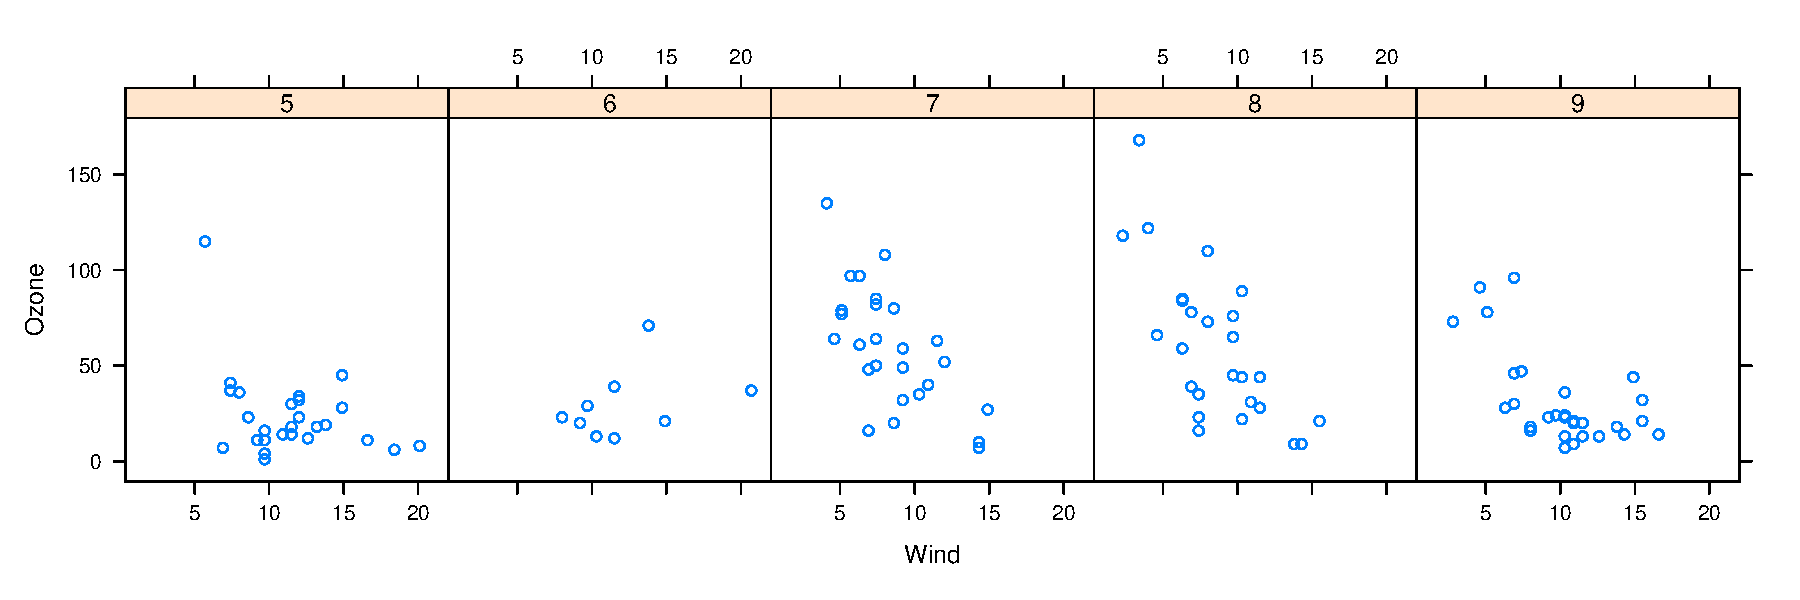
\includegraphics{semana_3_files/figure-latex/unnamed-chunk-2-1} \end{center}

\begin{itemize}
\tightlist
\item
  \textbf{Clasificación errónea:} \(1/16 = 0.06\)
\item
  \textbf{Gini:} \(1 - [(1/16) ^ 2 + (15/16) ^ 2] = 0.12\)
\item
  \textbf{Información:}
  \(- [1/16 \times log2 (1/16) + 15/16 \times log2 (15/16)] = 0.34\)
\end{itemize}

\begin{Shaded}
\begin{Highlighting}[]
\FunctionTok{par}\NormalTok{(}\AttributeTok{mar=}\FunctionTok{c}\NormalTok{(}\DecValTok{0}\NormalTok{,}\DecValTok{0}\NormalTok{,}\DecValTok{0}\NormalTok{,}\DecValTok{0}\NormalTok{)); }
\FunctionTok{plot}\NormalTok{(x,y,}\AttributeTok{xaxt=}\StringTok{"n"}\NormalTok{,}\AttributeTok{yaxt=}\StringTok{"n"}\NormalTok{,}\AttributeTok{cex=}\DecValTok{3}\NormalTok{,}\AttributeTok{col=}\FunctionTok{c}\NormalTok{(}\FunctionTok{rep}\NormalTok{(}\StringTok{"blue"}\NormalTok{,}\DecValTok{8}\NormalTok{),}\FunctionTok{rep}\NormalTok{(}\StringTok{"red"}\NormalTok{,}\DecValTok{8}\NormalTok{)),}\AttributeTok{pch=}\DecValTok{19}\NormalTok{)}
\end{Highlighting}
\end{Shaded}

\begin{center}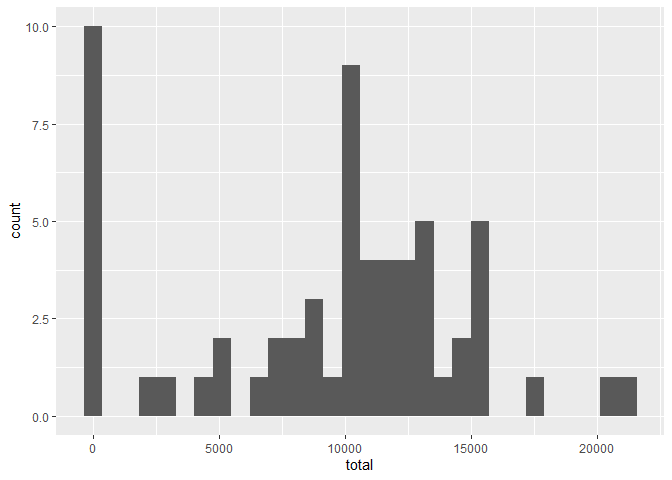
\includegraphics{semana_3_files/figure-latex/unnamed-chunk-3-1} \end{center}

\begin{itemize}
\tightlist
\item
  \textbf{Misclassification:} \(8/16 = 0.5\)
\item
  \textbf{Gini:} \(1 - [(8/16)^2 + (8/16)^2] = 0.5\)
\item
  \textbf{Information:}\(-[1/16 \times log2(1/16) + 15/16 \times log2(15/16)] = 1\)
\end{itemize}

ejemplo con datos iris

\begin{Shaded}
\begin{Highlighting}[]
\FunctionTok{library}\NormalTok{(caret)}
\FunctionTok{data}\NormalTok{(iris); }\FunctionTok{library}\NormalTok{(ggplot2)}
\FunctionTok{names}\NormalTok{(iris)}
\end{Highlighting}
\end{Shaded}

\begin{verbatim}
## [1] "Sepal.Length" "Sepal.Width"  "Petal.Length" "Petal.Width"  "Species"
\end{verbatim}

\begin{Shaded}
\begin{Highlighting}[]
\FunctionTok{table}\NormalTok{(iris}\SpecialCharTok{$}\NormalTok{Species)}
\end{Highlighting}
\end{Shaded}

\begin{verbatim}
## 
##     setosa versicolor  virginica 
##         50         50         50
\end{verbatim}

\begin{Shaded}
\begin{Highlighting}[]
\NormalTok{inTrain }\OtherTok{\textless{}{-}} \FunctionTok{createDataPartition}\NormalTok{(}\AttributeTok{y=}\NormalTok{iris}\SpecialCharTok{$}\NormalTok{Species,}
                              \AttributeTok{p=}\FloatTok{0.7}\NormalTok{, }\AttributeTok{list=}\ConstantTok{FALSE}\NormalTok{)}
\NormalTok{training }\OtherTok{\textless{}{-}}\NormalTok{ iris[inTrain,]}
\NormalTok{testing }\OtherTok{\textless{}{-}}\NormalTok{ iris[}\SpecialCharTok{{-}}\NormalTok{inTrain,]}
\FunctionTok{dim}\NormalTok{(training); }\FunctionTok{dim}\NormalTok{(testing)}
\end{Highlighting}
\end{Shaded}

\begin{verbatim}
## [1] 105   5
\end{verbatim}

\begin{verbatim}
## [1] 45  5
\end{verbatim}

hagaamos una grafica

\begin{Shaded}
\begin{Highlighting}[]
\FunctionTok{qplot}\NormalTok{(Petal.Width,Sepal.Width,}\AttributeTok{colour=}\NormalTok{Species,}\AttributeTok{data=}\NormalTok{training)}
\end{Highlighting}
\end{Shaded}

\begin{center}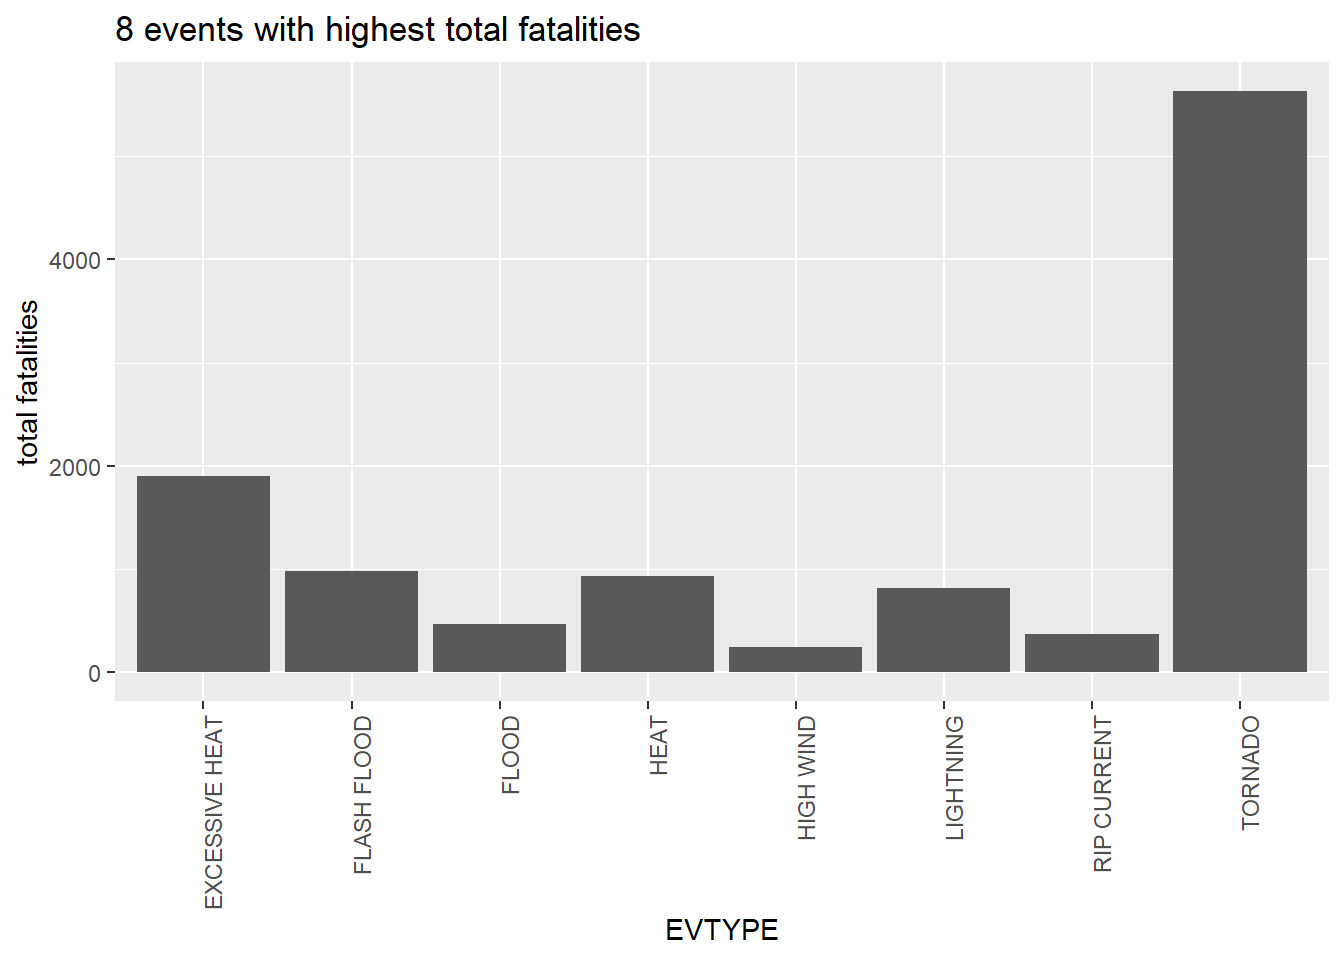
\includegraphics{semana_3_files/figure-latex/unnamed-chunk-5-1} \end{center}

podemos ver claramento que podemos hacer diviciones en la variable petal
width para predecir el tipo de especie, ahora hagamos un modelo para
predecir especies

\begin{Shaded}
\begin{Highlighting}[]
\NormalTok{modFit }\OtherTok{\textless{}{-}} \FunctionTok{train}\NormalTok{(Species }\SpecialCharTok{\textasciitilde{}}\NormalTok{ .,}\AttributeTok{method=}\StringTok{"rpart"}\NormalTok{,}\AttributeTok{data=}\NormalTok{training)}
\FunctionTok{print}\NormalTok{(modFit}\SpecialCharTok{$}\NormalTok{finalModel)}
\end{Highlighting}
\end{Shaded}

\begin{verbatim}
## n= 105 
## 
## node), split, n, loss, yval, (yprob)
##       * denotes terminal node
## 
## 1) root 105 70 setosa (0.33333333 0.33333333 0.33333333)  
##   2) Petal.Length< 2.35 35  0 setosa (1.00000000 0.00000000 0.00000000) *
##   3) Petal.Length>=2.35 70 35 versicolor (0.00000000 0.50000000 0.50000000)  
##     6) Petal.Width< 1.65 38  3 versicolor (0.00000000 0.92105263 0.07894737) *
##     7) Petal.Width>=1.65 32  0 virginica (0.00000000 0.00000000 1.00000000) *
\end{verbatim}

no es muy entendible que digamos, por eso lo graficamos

\begin{Shaded}
\begin{Highlighting}[]
\FunctionTok{plot}\NormalTok{(modFit}\SpecialCharTok{$}\NormalTok{finalModel, }\AttributeTok{uniform=}\ConstantTok{TRUE}\NormalTok{, }
      \AttributeTok{main=}\StringTok{"Classification Tree"}\NormalTok{)}
\FunctionTok{text}\NormalTok{(modFit}\SpecialCharTok{$}\NormalTok{finalModel, }\AttributeTok{use.n=}\ConstantTok{TRUE}\NormalTok{, }\AttributeTok{all=}\ConstantTok{TRUE}\NormalTok{, }\AttributeTok{cex=}\NormalTok{.}\DecValTok{8}\NormalTok{)}
\end{Highlighting}
\end{Shaded}

\begin{center}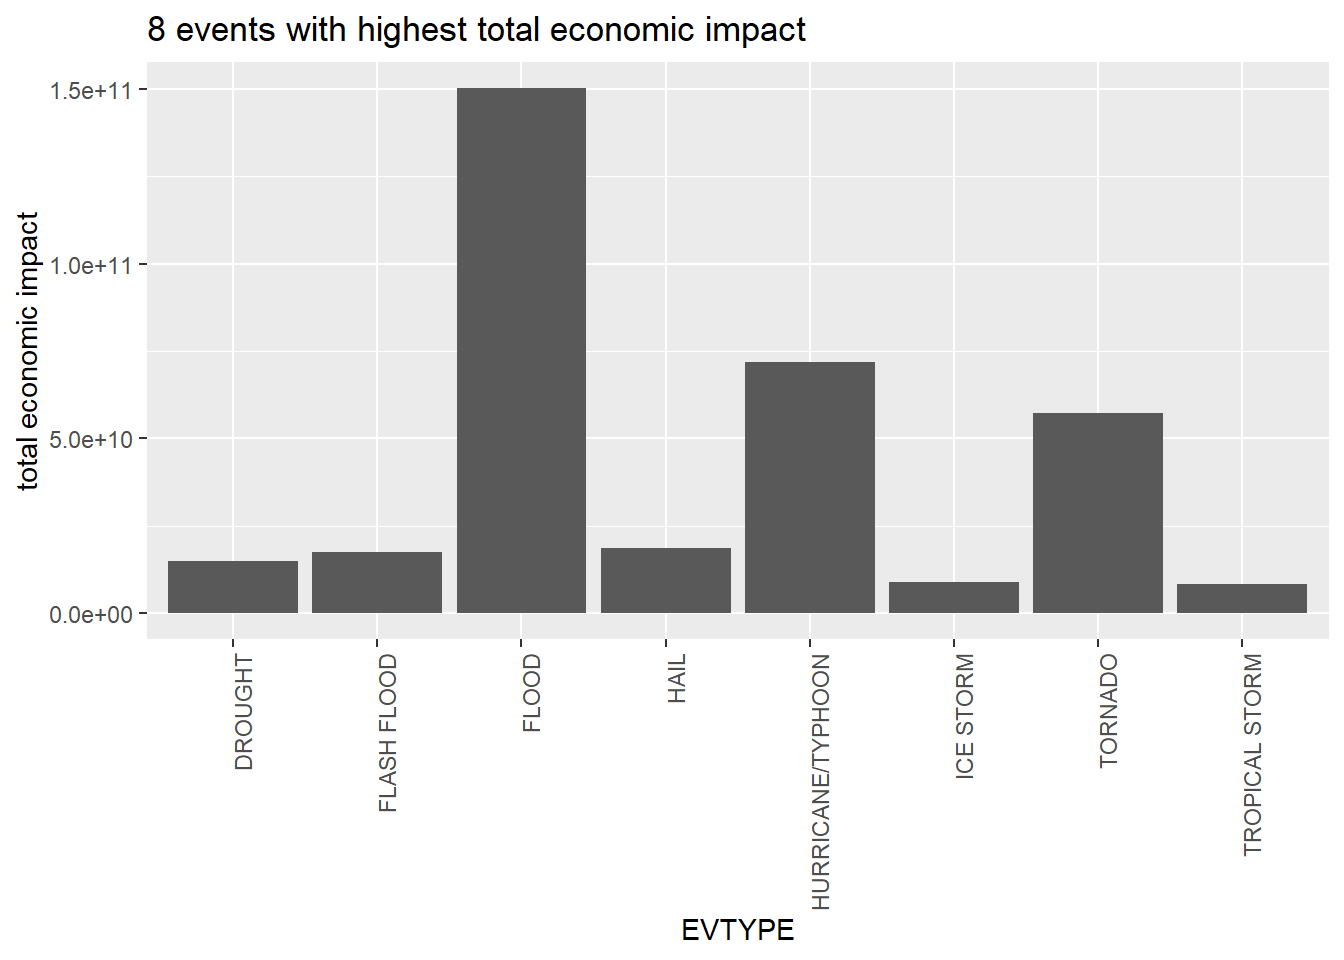
\includegraphics{semana_3_files/figure-latex/unnamed-chunk-7-1} \end{center}

\begin{Shaded}
\begin{Highlighting}[]
\FunctionTok{library}\NormalTok{(rattle)}
\FunctionTok{fancyRpartPlot}\NormalTok{(modFit}\SpecialCharTok{$}\NormalTok{finalModel)}
\end{Highlighting}
\end{Shaded}

\begin{center}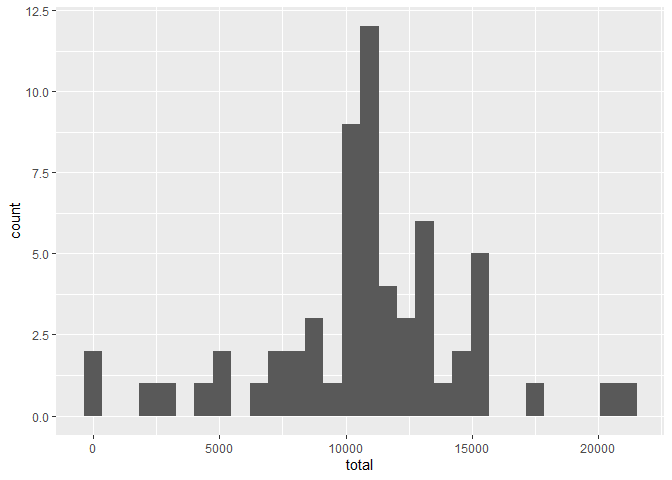
\includegraphics{semana_3_files/figure-latex/unnamed-chunk-8-1} \end{center}

prediciendo nuevos valores

\begin{Shaded}
\begin{Highlighting}[]
\FunctionTok{predict}\NormalTok{(modFit,}\AttributeTok{newdata=}\NormalTok{testing)}
\end{Highlighting}
\end{Shaded}

\begin{verbatim}
##  [1] setosa     setosa     setosa     setosa     setosa     setosa    
##  [7] setosa     setosa     setosa     setosa     setosa     setosa    
## [13] setosa     setosa     setosa     versicolor versicolor versicolor
## [19] versicolor versicolor versicolor versicolor virginica  versicolor
## [25] versicolor virginica  versicolor versicolor versicolor versicolor
## [31] virginica  virginica  virginica  virginica  virginica  virginica 
## [37] versicolor virginica  virginica  virginica  virginica  virginica 
## [43] virginica  virginica  virginica 
## Levels: setosa versicolor virginica
\end{verbatim}

\hypertarget{notas-y-recursos-adicionales}{%
\subsection{Notas y recursos
adicionales}\label{notas-y-recursos-adicionales}}

\begin{itemize}
\tightlist
\item
  Los árboles de clasificación son modelos no lineales

  \begin{itemize}
  \tightlist
  \item
    Usan interacciones entre variables
  \item
    Las transformaciones de datos pueden ser menos importantes
    (transformaciones monótonas)
  \item
    Los árboles también se pueden utilizar para problemas de regresión
    (resultado continuo)
  \end{itemize}
\item
  Tenga en cuenta que hay varias opciones de construcción de árboles en
  R tanto en el paquete de intercalación:
  \href{http://cran.r-project.org/web/packages/party/index.html}{party},
  \href{http://cran.r-project.org/web/packages/rpart/index.html}{rpart}
  y fuera del paquete caret -
  \href{http://cran.r-project.org/web/packages/tree/index.html}{tree}
\item
  \href{http://www-bcf.usc.edu/~gareth/ISL/}{Introducción al aprendizaje
  estadístico}
\item
  \href{http://www-stat.stanford.edu/~tibs/ElemStatLearn/}{Elementos de
  aprendizaje estadístico}
\item
  \href{http://www.amazon.com/Classification-Regression-Trees-Leo-Breiman/dp/0412048418}{Árboles
  de clasificación y regresión} \# bagging
\end{itemize}

\textbf{Idea básica}:

\begin{enumerate}
\def\labelenumi{\arabic{enumi}.}
\tightlist
\item
  Volver a muestrear casos y volver a calcular las predicciones
\item
  Voto medio o mayoritario
\end{enumerate}

\textbf{Notas}:

\begin{itemize}
\tightlist
\item
  Sesgo similar
\item
  Varianza reducida
\item
  Más útil para funciones no lineales
\end{itemize}

ejemplo con datos ozono

\begin{Shaded}
\begin{Highlighting}[]
\FunctionTok{data}\NormalTok{(airquality)}
\NormalTok{ozone}\OtherTok{\textless{}{-}}\NormalTok{airquality}
\FunctionTok{names}\NormalTok{(ozone)}\OtherTok{\textless{}{-}}\FunctionTok{c}\NormalTok{(}\StringTok{"ozone"}\NormalTok{,}\StringTok{"Solar.R"}\NormalTok{, }\StringTok{"Wind"}\NormalTok{, }\StringTok{"temperature"}\NormalTok{, }\StringTok{"Month"}\NormalTok{,}\StringTok{"Day"}\NormalTok{)}
\FunctionTok{head}\NormalTok{(ozone)}
\end{Highlighting}
\end{Shaded}

\begin{verbatim}
##   ozone Solar.R Wind temperature Month Day
## 1    41     190  7.4          67     5   1
## 2    36     118  8.0          72     5   2
## 3    12     149 12.6          74     5   3
## 4    18     313 11.5          62     5   4
## 5    NA      NA 14.3          56     5   5
## 6    28      NA 14.9          66     5   6
\end{verbatim}

\begin{Shaded}
\begin{Highlighting}[]
\NormalTok{ll }\OtherTok{\textless{}{-}} \FunctionTok{matrix}\NormalTok{(}\ConstantTok{NA}\NormalTok{,}\AttributeTok{nrow=}\DecValTok{10}\NormalTok{,}\AttributeTok{ncol=}\DecValTok{155}\NormalTok{)}
\ControlFlowTok{for}\NormalTok{(i }\ControlFlowTok{in} \DecValTok{1}\SpecialCharTok{:}\DecValTok{10}\NormalTok{)\{}
\NormalTok{  ss }\OtherTok{\textless{}{-}} \FunctionTok{sample}\NormalTok{(}\DecValTok{1}\SpecialCharTok{:}\FunctionTok{dim}\NormalTok{(ozone)[}\DecValTok{1}\NormalTok{],}\AttributeTok{replace=}\NormalTok{T)}
\NormalTok{  ozone0 }\OtherTok{\textless{}{-}}\NormalTok{ ozone[ss,]; ozone0 }\OtherTok{\textless{}{-}}\NormalTok{ ozone0[}\FunctionTok{order}\NormalTok{(ozone0}\SpecialCharTok{$}\NormalTok{ozone),]}
\NormalTok{  loess0 }\OtherTok{\textless{}{-}} \FunctionTok{loess}\NormalTok{(temperature }\SpecialCharTok{\textasciitilde{}}\NormalTok{ ozone,}\AttributeTok{data=}\NormalTok{ozone0,}\AttributeTok{span=}\FloatTok{0.2}\NormalTok{)}
\NormalTok{  ll[i,] }\OtherTok{\textless{}{-}} \FunctionTok{predict}\NormalTok{(loess0,}\AttributeTok{newdata=}\FunctionTok{data.frame}\NormalTok{(}\AttributeTok{ozone=}\DecValTok{1}\SpecialCharTok{:}\DecValTok{155}\NormalTok{))}
\NormalTok{\}}
\end{Highlighting}
\end{Shaded}

graficando, la roja es la ``media''

\begin{Shaded}
\begin{Highlighting}[]
\FunctionTok{plot}\NormalTok{(ozone}\SpecialCharTok{$}\NormalTok{ozone,ozone}\SpecialCharTok{$}\NormalTok{temperature,}\AttributeTok{pch=}\DecValTok{19}\NormalTok{,}\AttributeTok{cex=}\FloatTok{0.5}\NormalTok{)}
\ControlFlowTok{for}\NormalTok{(i }\ControlFlowTok{in} \DecValTok{1}\SpecialCharTok{:}\DecValTok{10}\NormalTok{)\{}\FunctionTok{lines}\NormalTok{(}\DecValTok{1}\SpecialCharTok{:}\DecValTok{155}\NormalTok{,ll[i,],}\AttributeTok{col=}\StringTok{"grey"}\NormalTok{,}\AttributeTok{lwd=}\DecValTok{2}\NormalTok{)\}}
\FunctionTok{lines}\NormalTok{(}\DecValTok{1}\SpecialCharTok{:}\DecValTok{155}\NormalTok{,}\FunctionTok{apply}\NormalTok{(ll,}\DecValTok{2}\NormalTok{,mean),}\AttributeTok{col=}\StringTok{"red"}\NormalTok{,}\AttributeTok{lwd=}\DecValTok{2}\NormalTok{)}
\end{Highlighting}
\end{Shaded}

\begin{center}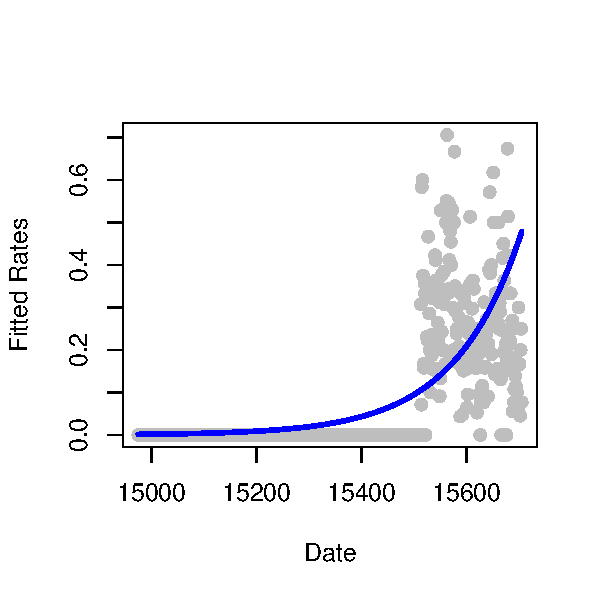
\includegraphics{semana_3_files/figure-latex/unnamed-chunk-12-1} \end{center}

\emph{con caret}

\begin{itemize}
\tightlist
\item
  Algunos modelos realizan el baggin por usted, en la función
  \texttt{train} considere las opciones de \texttt{method}

  \begin{itemize}
  \tightlist
  \item
    \texttt{bagEarth}
  \item
    \texttt{treebag}
  \item
    \texttt{bagFDA}
  \end{itemize}
\item
  Alternativamente, puede hacer baggin en cualquier modelo que elija
  utilizando la función \texttt{bag}
\end{itemize}

\begin{Shaded}
\begin{Highlighting}[]
\NormalTok{predictors }\OtherTok{=} \FunctionTok{data.frame}\NormalTok{(}\AttributeTok{ozone=}\NormalTok{ozone}\SpecialCharTok{$}\NormalTok{ozone)}
\NormalTok{temperature }\OtherTok{=}\NormalTok{ ozone}\SpecialCharTok{$}\NormalTok{temperature}
\NormalTok{treebag }\OtherTok{\textless{}{-}} \FunctionTok{bag}\NormalTok{(predictors, temperature, }\AttributeTok{B =} \DecValTok{10}\NormalTok{,}
                \AttributeTok{bagControl =} \FunctionTok{bagControl}\NormalTok{(}\AttributeTok{fit =}\NormalTok{ ctreeBag}\SpecialCharTok{$}\NormalTok{fit,}
                                        \AttributeTok{predict =}\NormalTok{ ctreeBag}\SpecialCharTok{$}\NormalTok{pred,}
                                        \AttributeTok{aggregate =}\NormalTok{ ctreeBag}\SpecialCharTok{$}\NormalTok{aggregate))}

\FunctionTok{plot}\NormalTok{(ozone}\SpecialCharTok{$}\NormalTok{ozone,temperature,}\AttributeTok{col=}\StringTok{\textquotesingle{}lightgrey\textquotesingle{}}\NormalTok{,}\AttributeTok{pch=}\DecValTok{19}\NormalTok{)}
\FunctionTok{points}\NormalTok{(ozone}\SpecialCharTok{$}\NormalTok{ozone,}\FunctionTok{predict}\NormalTok{(treebag}\SpecialCharTok{$}\NormalTok{fits[[}\DecValTok{1}\NormalTok{]]}\SpecialCharTok{$}\NormalTok{fit,predictors),}\AttributeTok{pch=}\DecValTok{19}\NormalTok{,}\AttributeTok{col=}\StringTok{"red"}\NormalTok{)}
\FunctionTok{points}\NormalTok{(ozone}\SpecialCharTok{$}\NormalTok{ozone,}\FunctionTok{predict}\NormalTok{(treebag,predictors),}\AttributeTok{pch=}\DecValTok{19}\NormalTok{,}\AttributeTok{col=}\StringTok{"blue"}\NormalTok{)}
\end{Highlighting}
\end{Shaded}

\begin{center}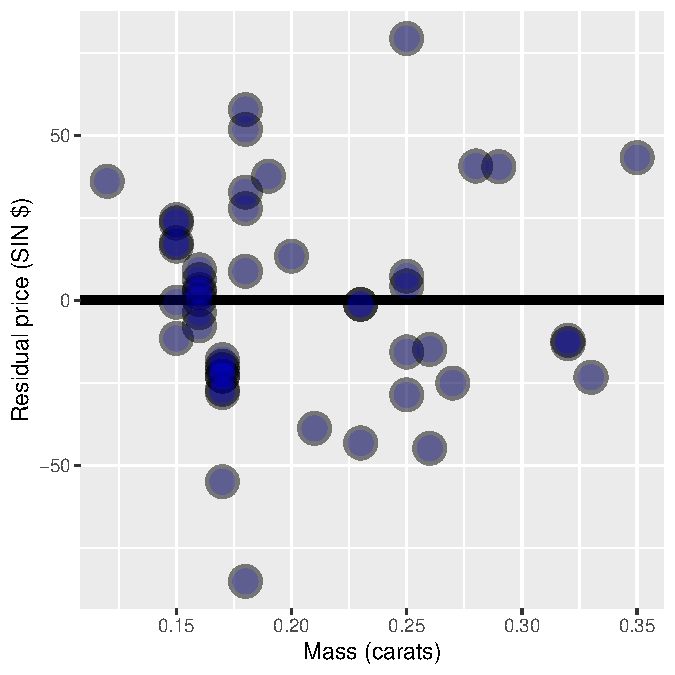
\includegraphics{semana_3_files/figure-latex/unnamed-chunk-13-1} \end{center}

partes de baggin con caret

\begin{Shaded}
\begin{Highlighting}[]
\NormalTok{ctreeBag}\SpecialCharTok{$}\NormalTok{fit}
\end{Highlighting}
\end{Shaded}

\begin{verbatim}
## function (x, y, ...) 
## {
##     loadNamespace("party")
##     data <- as.data.frame(x, stringsAsFactors = TRUE)
##     data$y <- y
##     party::ctree(y ~ ., data = data)
## }
## <bytecode: 0x00000000275667a0>
## <environment: namespace:caret>
\end{verbatim}

\begin{Shaded}
\begin{Highlighting}[]
\NormalTok{ctreeBag}\SpecialCharTok{$}\NormalTok{pred}
\end{Highlighting}
\end{Shaded}

\begin{verbatim}
## function (object, x) 
## {
##     if (!is.data.frame(x)) 
##         x <- as.data.frame(x, stringsAsFactors = TRUE)
##     obsLevels <- levels(object@data@get("response")[, 1])
##     if (!is.null(obsLevels)) {
##         rawProbs <- party::treeresponse(object, x)
##         probMatrix <- matrix(unlist(rawProbs), ncol = length(obsLevels), 
##             byrow = TRUE)
##         out <- data.frame(probMatrix)
##         colnames(out) <- obsLevels
##         rownames(out) <- NULL
##     }
##     else out <- unlist(party::treeresponse(object, x))
##     out
## }
## <bytecode: 0x00000000275671e8>
## <environment: namespace:caret>
\end{verbatim}

\begin{Shaded}
\begin{Highlighting}[]
\NormalTok{ctreeBag}\SpecialCharTok{$}\NormalTok{aggregate}
\end{Highlighting}
\end{Shaded}

\begin{verbatim}
## function (x, type = "class") 
## {
##     if (is.matrix(x[[1]]) | is.data.frame(x[[1]])) {
##         pooled <- x[[1]] & NA
##         classes <- colnames(pooled)
##         for (i in 1:ncol(pooled)) {
##             tmp <- lapply(x, function(y, col) y[, col], col = i)
##             tmp <- do.call("rbind", tmp)
##             pooled[, i] <- apply(tmp, 2, median)
##         }
##         if (type == "class") {
##             out <- factor(classes[apply(pooled, 1, which.max)], 
##                 levels = classes)
##         }
##         else out <- as.data.frame(pooled, stringsAsFactors = TRUE)
##     }
##     else {
##         x <- matrix(unlist(x), ncol = length(x))
##         out <- apply(x, 1, median)
##     }
##     out
## }
## <bytecode: 0x0000000027565178>
## <environment: namespace:caret>
\end{verbatim}

\hypertarget{notas-y-otros-recursos}{%
\subsection{Notas y otros recursos}\label{notas-y-otros-recursos}}

\textbf{Notas}:

\begin{itemize}
\tightlist
\item
  El bagging es más útil para modelos no lineales
\item
  Se usa a menudo con árboles: una extensión son bosques aleatorios
\item
  Varios modelos utilizan bagging en la función \emph{train} de caret
\end{itemize}

\textbf{Otros recursos}:

\begin{itemize}
\tightlist
\item
  \href{http://en.wikipedia.org/wiki/Bootstrap_aggregating}{Embolsado}
\item
  \href{http://stat.ethz.ch/education/semesters/FS_2008/CompStat/sk-ch8.pdf}{Embolsado
  y boosting}
\item
  \href{http://www-stat.stanford.edu/~tibs/ElemStatLearn/}{Elementos de
  aprendizaje estadístico}
\end{itemize}

\hypertarget{random-forests}{%
\section{Random forests}\label{random-forests}}

\begin{enumerate}
\def\labelenumi{\arabic{enumi}.}
\tightlist
\item
  Muestras de Bootstrap
\item
  En cada división, las variables de arranque
\item
  Cultiva varios árboles y vota
\end{enumerate}

\textbf{Pros}:

\begin{enumerate}
\def\labelenumi{\arabic{enumi}.}
\tightlist
\item
  Precisión
\end{enumerate}

\textbf{Contras}:

\begin{enumerate}
\def\labelenumi{\arabic{enumi}.}
\tightlist
\item
  Velocidad
\item
  Interpretabilidad
\item
  Sobreajuste
\end{enumerate}

\begin{center}\includegraphics[width=1\linewidth]{D:/luism/Documents/courses/assets/img/08_PredictionAndMachineLearning/forests} \end{center}

ejemplo con datos iris

\begin{Shaded}
\begin{Highlighting}[]
\FunctionTok{data}\NormalTok{(iris); }\FunctionTok{library}\NormalTok{(ggplot2);}\FunctionTok{library}\NormalTok{(caret)}
\NormalTok{inTrain }\OtherTok{\textless{}{-}} \FunctionTok{createDataPartition}\NormalTok{(}\AttributeTok{y=}\NormalTok{iris}\SpecialCharTok{$}\NormalTok{Species,}
                              \AttributeTok{p=}\FloatTok{0.7}\NormalTok{, }\AttributeTok{list=}\ConstantTok{FALSE}\NormalTok{)}
\NormalTok{training }\OtherTok{\textless{}{-}}\NormalTok{ iris[inTrain,]}
\NormalTok{testing }\OtherTok{\textless{}{-}}\NormalTok{ iris[}\SpecialCharTok{{-}}\NormalTok{inTrain,]}


\NormalTok{modFit }\OtherTok{\textless{}{-}} \FunctionTok{train}\NormalTok{(Species}\SpecialCharTok{\textasciitilde{}}\NormalTok{ .,}\AttributeTok{data=}\NormalTok{training,}\AttributeTok{method=}\StringTok{"rf"}\NormalTok{,}\AttributeTok{prox=}\ConstantTok{TRUE}\NormalTok{)}
\NormalTok{modFit}
\end{Highlighting}
\end{Shaded}

\begin{verbatim}
## Random Forest 
## 
## 105 samples
##   4 predictor
##   3 classes: 'setosa', 'versicolor', 'virginica' 
## 
## No pre-processing
## Resampling: Bootstrapped (25 reps) 
## Summary of sample sizes: 105, 105, 105, 105, 105, 105, ... 
## Resampling results across tuning parameters:
## 
##   mtry  Accuracy   Kappa    
##   2     0.9423389  0.9118121
##   3     0.9404694  0.9090803
##   4     0.9377160  0.9050166
## 
## Accuracy was used to select the optimal model using the largest value.
## The final value used for the model was mtry = 2.
\end{verbatim}

Conseguir un solo árbol

\begin{Shaded}
\begin{Highlighting}[]
\FunctionTok{library}\NormalTok{(randomForest)}
\FunctionTok{getTree}\NormalTok{(modFit}\SpecialCharTok{$}\NormalTok{finalModel,}\AttributeTok{k=}\DecValTok{2}\NormalTok{)}
\end{Highlighting}
\end{Shaded}

\begin{verbatim}
##    left daughter right daughter split var split point status prediction
## 1              2              3         3        2.50      1          0
## 2              0              0         0        0.00     -1          1
## 3              4              5         3        4.85      1          0
## 4              6              7         4        1.65      1          0
## 5              8              9         4        1.70      1          0
## 6              0              0         0        0.00     -1          2
## 7              0              0         0        0.00     -1          3
## 8             10             11         4        1.55      1          0
## 9              0              0         0        0.00     -1          3
## 10            12             13         3        4.95      1          0
## 11             0              0         0        0.00     -1          2
## 12             0              0         0        0.00     -1          2
## 13             0              0         0        0.00     -1          3
\end{verbatim}

Creando prototipos (son los taches), Los prototipos son casos
``representativos'' de un grupo de puntos de datos, dada la matriz de
similitud entre los puntos. Son muy similares a los medoides.

\begin{Shaded}
\begin{Highlighting}[]
\NormalTok{irisP }\OtherTok{\textless{}{-}} \FunctionTok{classCenter}\NormalTok{(training[,}\FunctionTok{c}\NormalTok{(}\DecValTok{3}\NormalTok{,}\DecValTok{4}\NormalTok{)], training}\SpecialCharTok{$}\NormalTok{Species, modFit}\SpecialCharTok{$}\NormalTok{finalModel}\SpecialCharTok{$}\NormalTok{prox)}
\NormalTok{irisP }\OtherTok{\textless{}{-}} \FunctionTok{as.data.frame}\NormalTok{(irisP); irisP}\SpecialCharTok{$}\NormalTok{Species }\OtherTok{\textless{}{-}} \FunctionTok{rownames}\NormalTok{(irisP)}
\NormalTok{p }\OtherTok{\textless{}{-}} \FunctionTok{qplot}\NormalTok{(Petal.Width, Petal.Length, }\AttributeTok{col=}\NormalTok{Species,}\AttributeTok{data=}\NormalTok{training)}
\NormalTok{p }\SpecialCharTok{+} \FunctionTok{geom\_point}\NormalTok{(}\FunctionTok{aes}\NormalTok{(}\AttributeTok{x=}\NormalTok{Petal.Width,}\AttributeTok{y=}\NormalTok{Petal.Length,}\AttributeTok{col=}\NormalTok{Species),}\AttributeTok{size=}\DecValTok{5}\NormalTok{,}\AttributeTok{shape=}\DecValTok{4}\NormalTok{,}\AttributeTok{data=}\NormalTok{irisP)}
\end{Highlighting}
\end{Shaded}

\begin{center}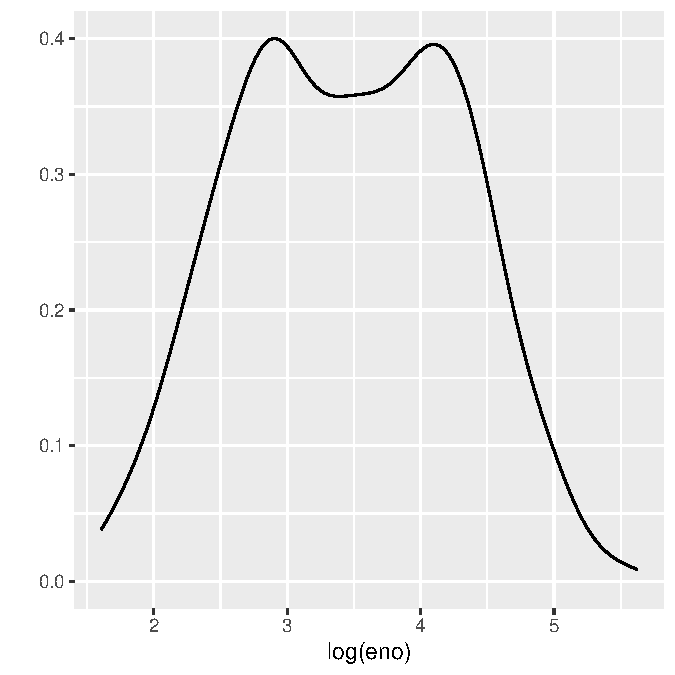
\includegraphics{semana_3_files/figure-latex/unnamed-chunk-18-1} \end{center}

prediciendo nuevos valores

\begin{Shaded}
\begin{Highlighting}[]
\NormalTok{pred }\OtherTok{\textless{}{-}} \FunctionTok{predict}\NormalTok{(modFit,testing); testing}\SpecialCharTok{$}\NormalTok{predRight }\OtherTok{\textless{}{-}}\NormalTok{ pred}\SpecialCharTok{==}\NormalTok{testing}\SpecialCharTok{$}\NormalTok{Species}
\FunctionTok{table}\NormalTok{(pred,testing}\SpecialCharTok{$}\NormalTok{Species)}
\end{Highlighting}
\end{Shaded}

\begin{verbatim}
##             
## pred         setosa versicolor virginica
##   setosa         15          0         0
##   versicolor      0         14         3
##   virginica       0          1        12
\end{verbatim}

\begin{Shaded}
\begin{Highlighting}[]
\FunctionTok{qplot}\NormalTok{(Petal.Width,Petal.Length,}\AttributeTok{colour=}\NormalTok{predRight,}\AttributeTok{data=}\NormalTok{testing,}\AttributeTok{main=}\StringTok{"newdata Predictions"}\NormalTok{)}
\end{Highlighting}
\end{Shaded}

\begin{center}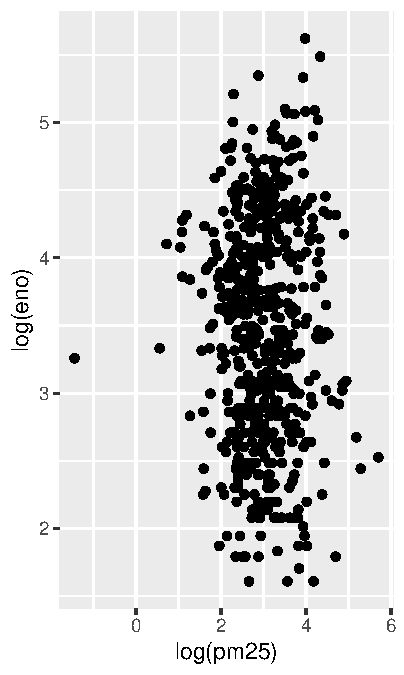
\includegraphics{semana_3_files/figure-latex/unnamed-chunk-19-1} \end{center}

\hypertarget{notas-y-otros-recursos-1}{%
\subsection{Notas y otros recursos}\label{notas-y-otros-recursos-1}}

\textbf{Notas}:

\begin{itemize}
\tightlist
\item
  Los bosques aleatorios suelen ser uno de los dos algoritmos de mejor
  rendimiento junto con el boosting en los concursos de predicción.
\item
  Los bosques aleatorios son difíciles de interpretar pero a menudo muy
  precisos.
\item
  Se debe tener cuidado para evitar el sobreajuste (consulte la función
  \href{http://cran.r-project.org/web/packages/randomForest/randomForest.pdf}{rfcv})
\end{itemize}

\textbf{Otros recursos}:

\begin{itemize}
\tightlist
\item
  \href{http://www.stat.berkeley.edu/~breiman/RandomForests/cc_home.htm}{Bosques
  aleatorios}
\item
  \href{http://en.wikipedia.org/wiki/Random_forest}{Wikipedia del bosque
  aleatorio}
\item
  \href{http://www-stat.stanford.edu/~tibs/ElemStatLearn/}{Elementos de
  aprendizaje estadístico}
\end{itemize}

\hypertarget{boosting}{%
\section{boosting}\label{boosting}}

Idea básica

\begin{enumerate}
\def\labelenumi{\arabic{enumi}.}
\tightlist
\item
  Tome muchos predictores (posiblemente) débiles
\item
  Péselos y súmelos
\item
  Obtenga un predictor más fuerte
\end{enumerate}

Idea básica detrás del iboosting

\begin{enumerate}
\def\labelenumi{\arabic{enumi}.}
\tightlist
\item
  Comience con un conjunto de clasificadores \(h_1, \ldots, h_k\)

  \begin{itemize}
  \tightlist
  \item
    Ejemplos: todos los árboles posibles, todos los modelos de regresión
    posibles, todos los cortes posibles.
  \end{itemize}
\item
  Cree un clasificador que combine funciones de clasificación:
  \(f(x) = \rm{sgn}\left(\sum_{t=1}^T \alpha_t h_t(x)\right)\)..

  \begin{itemize}
  \tightlist
  \item
    El objetivo es minimizar el error (en el conjunto de entrenamiento)
  \item
    Iterativo, seleccione un \(h\) en cada paso
  \item
    Calcular pesos basados en errores
  \item
    Subir clasificaciones perdidas y seleccionar los siguientes \(h\)
  \end{itemize}
\end{enumerate}

ejemplo simple, se trada de crear un clasificador que clasifique entre
\textcolor{red}{-} y \textcolor{blue}{+}

\begin{center}\includegraphics[width=1\linewidth]{D:/luism/Documents/courses/assets/img/08_PredictionAndMachineLearning/ada1} \end{center}

el primer clasificador es una linea vertical

\begin{center}\includegraphics[width=1\linewidth]{D:/luism/Documents/courses/assets/img/08_PredictionAndMachineLearning/adar1} \end{center}

para el segundo y tercer clasificador se crea una linea vertical y
horizontal

\begin{center}\includegraphics[width=1\linewidth]{D:/luism/Documents/courses/assets/img/08_PredictionAndMachineLearning/ada2} \end{center}

se combinan los 3 predictores

\begin{center}\includegraphics[width=1\linewidth]{D:/luism/Documents/courses/assets/img/08_PredictionAndMachineLearning/ada3} \end{center}

boosting en R

\begin{itemize}
\tightlist
\item
  El boosting se puede usar con cualquier subconjunto de clasificadores
\item
  Una gran subclase es
  \href{http://en.wikipedia.org/wiki/Gradient_boosting}{aumento de
  gradiente}
\item
  R tiene múltiples bibliotecas de boosting. Las diferencias incluyen la
  elección de funciones básicas de clasificación y reglas de
  combinación.

  \begin{itemize}
  \tightlist
  \item
    \href{http://cran.r-project.org/web/packages/gbm/index.html}{gbm}:
    boosting con árboles.
  \item
    \href{http://cran.r-project.org/web/packages/mboost/index.html}{mboost}:
    boosting basado en modelos
  \item
    \href{http://cran.r-project.org/web/packages/ada/index.html}{ada} -
    boosting estadístico basado en
    \href{http://projecteuclid.org/DPubS?service=\%20UI\%20\&\%20version\%20=\%201.0\%20\&\%20verb\%20=\%20Display\%20\&\%20handle\%20=\%20euclid.aos\%20/\%201016218223}{regresión
    logística aditiva}
  \item
    \href{http://cran.r-project.org/web/packages/GAMBoost/index.html}{gamBoost}
    para impulsar modelos aditivos generalizados
  \end{itemize}
\item
  La mayoría de estos están disponibles en el paquete de caret.
\end{itemize}

ejemplo con datos de sueldo

\begin{Shaded}
\begin{Highlighting}[]
\FunctionTok{library}\NormalTok{(ISLR); }\FunctionTok{data}\NormalTok{(Wage); }\FunctionTok{library}\NormalTok{(ggplot2); }\FunctionTok{library}\NormalTok{(caret);}
\NormalTok{Wage }\OtherTok{\textless{}{-}} \FunctionTok{subset}\NormalTok{(Wage,}\AttributeTok{select=}\SpecialCharTok{{-}}\FunctionTok{c}\NormalTok{(logwage))}
\NormalTok{inTrain }\OtherTok{\textless{}{-}} \FunctionTok{createDataPartition}\NormalTok{(}\AttributeTok{y=}\NormalTok{Wage}\SpecialCharTok{$}\NormalTok{wage,}
                              \AttributeTok{p=}\FloatTok{0.7}\NormalTok{, }\AttributeTok{list=}\ConstantTok{FALSE}\NormalTok{)}
\NormalTok{training }\OtherTok{\textless{}{-}}\NormalTok{ Wage[inTrain,]; testing }\OtherTok{\textless{}{-}}\NormalTok{ Wage[}\SpecialCharTok{{-}}\NormalTok{inTrain,]}

\NormalTok{modFit }\OtherTok{\textless{}{-}} \FunctionTok{train}\NormalTok{(wage }\SpecialCharTok{\textasciitilde{}}\NormalTok{ ., }\AttributeTok{method=}\StringTok{"gbm"}\NormalTok{,}\AttributeTok{data=}\NormalTok{training,}\AttributeTok{verbose=}\ConstantTok{FALSE}\NormalTok{)}
\FunctionTok{print}\NormalTok{(modFit)}
\end{Highlighting}
\end{Shaded}

\begin{verbatim}
## Stochastic Gradient Boosting 
## 
## 2102 samples
##    9 predictor
## 
## No pre-processing
## Resampling: Bootstrapped (25 reps) 
## Summary of sample sizes: 2102, 2102, 2102, 2102, 2102, 2102, ... 
## Resampling results across tuning parameters:
## 
##   interaction.depth  n.trees  RMSE      Rsquared   MAE     
##   1                   50      34.02735  0.3164369  23.17244
##   1                  100      33.48048  0.3268483  22.80521
##   1                  150      33.41638  0.3283001  22.81330
##   2                   50      33.53075  0.3260401  22.81065
##   2                  100      33.43372  0.3280820  22.86149
##   2                  150      33.49621  0.3264654  22.95321
##   3                   50      33.39058  0.3299187  22.74033
##   3                  100      33.56036  0.3242165  22.96235
##   3                  150      33.77585  0.3179243  23.15347
## 
## Tuning parameter 'shrinkage' was held constant at a value of 0.1
## 
## Tuning parameter 'n.minobsinnode' was held constant at a value of 10
## RMSE was used to select the optimal model using the smallest value.
## The final values used for the model were n.trees = 50, interaction.depth =
##  3, shrinkage = 0.1 and n.minobsinnode = 10.
\end{verbatim}

\begin{Shaded}
\begin{Highlighting}[]
\FunctionTok{qplot}\NormalTok{(}\FunctionTok{predict}\NormalTok{(modFit,testing),wage,}\AttributeTok{data=}\NormalTok{testing)}
\end{Highlighting}
\end{Shaded}

\begin{center}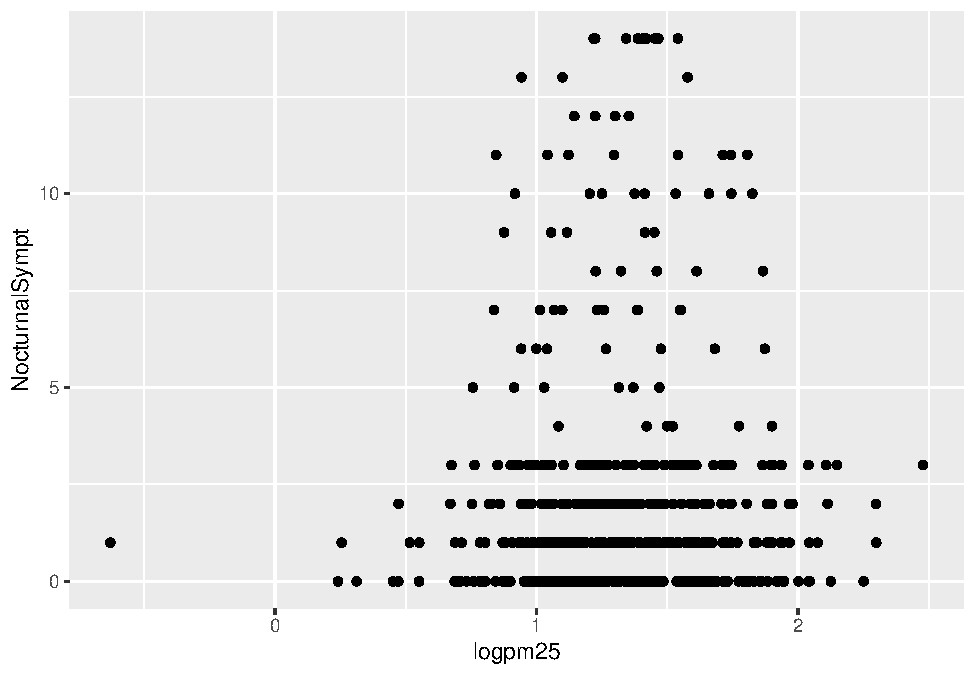
\includegraphics{semana_3_files/figure-latex/unnamed-chunk-25-1} \end{center}

\hypertarget{notas-y-lectura-adicional}{%
\subsection{Notas y lectura adicional}\label{notas-y-lectura-adicional}}

\begin{itemize}
\tightlist
\item
  Un par de buenos tutoriales para impulsar

  \begin{itemize}
  \tightlist
  \item
    Freund y Shapire -
    \href{http://www.cc.gatech.edu/~thad/6601-gradAI\%20-fall2013\%20/\%20boosting.pdf}{http://www.cc.gatech.edu/\textasciitilde thad/6601-gradAI-fall2013/boosting.pdf}
  \item
    Ron Meir-
    \url{http://webee.technion.ac.il/people/rmeir/BoostingTutorial.pdf}
  \end{itemize}
\item
  boosting, bosques aleatorios y conjuntos de modelos son las
  herramientas más comunes que ganan Kaggle y otros concursos de
  predicción.

  \begin{itemize}
  \tightlist
  \item
    \url{http://www.netflixprize.com/assets/GrandPrize2009_BPC_BigChaos.pdf}
  \item
    \url{https://kaggle2.blob.core.windows.net/wiki-files/327/09ccf652-8c1c-4a3d-b979-ce2369c985e4/Willem\%20Mestrom\%20-\%20Milestone\%201\%20Description\%20V2\%202.pdf}
    *\href{http://en.wikipedia.org/wiki/AdaBoost}{Adaboost on Wikipedia}
  \end{itemize}
\end{itemize}

\hypertarget{prediccion-basada-en-modelos}{%
\section{prediccion basada en
modelos}\label{prediccion-basada-en-modelos}}

\emph{Idea básica}

\begin{enumerate}
\def\labelenumi{\arabic{enumi}.}
\tightlist
\item
  Suponga que los datos siguen un modelo probabilístico
\item
  Utilice el teorema de Bayes para identificar clasificadores óptimos
\end{enumerate}

\textbf{Pros: }

\begin{itemize}
\tightlist
\item
  Puede aprovechar la estructura de los datos.
\item
  Puede ser conveniente computacionalmente
\item
  Son razonablemente precisos en problemas reales.
\end{itemize}

\textbf{Contras:}

\begin{itemize}
\tightlist
\item
  Haga suposiciones adicionales sobre los datos
\item
  Cuando el modelo es incorrecto, es posible que se reduzca la precisión
\end{itemize}

\begin{enumerate}
\def\labelenumi{\arabic{enumi}.}
\item
  Nuestro objetivo es construir un modelo paramétrico para distribución
  condicional \(P(Y = k | X = x)\)
\item
  Un enfoque típico es aplicar el
  \href{http://en.wikipedia.org/wiki/Bayes'_theorem}{teorema de Bayes}:
  \[Pr(Y = k | X=x) = \frac{Pr(X=x|Y=k)Pr(Y=k)}{\sum_{\ell=1}^K Pr(X=x |Y = \ell) Pr(Y=\ell)}\]
  \[Pr(Y = k | X=x) = \frac{f_k(x) \pi_k}{\sum_{\ell = 1}^K f_{\ell}(x) \pi_{\ell}}\]
\item
  Normalmente, las probabilidades priori \(\pi_k\) se establecen de
  antemano.
\item
  Una elección común para
  \(f_k(x) = \frac{1}{\sigma_k \sqrt{2 \pi}}e^{-\frac{(x-\mu_k)^2}{\sigma_k^2}}\),
  la distribucion normal
\item
  Estimar los parametros de (\(\mu_k\),\(\sigma_k^2\))
\item
  Clasifique en la clase con el valor más alto de \(P(Y = k | X = x)\)
\end{enumerate}

Una variedad de modelos utilizan este enfoque

\begin{itemize}
\tightlist
\item
  El análisis discriminante lineal supone que \(f_k (x)\) es gaussiano
  multivariante con las mismas covarianzas
\item
  El análisis discriminatorio cuadrático asume que \(f_k (x)\) es
  gaussiano multivariante con diferentes covarianzas
\item
  \href{http://www.stat.washington.edu/mclust/}{Predicción basada en
  modelos} asume versiones más complicadas para la matriz de covarianza
\item
  Naive Bayes asume la independencia entre características para la
  construcción de modelos
\end{itemize}

\url{http://statweb.stanford.edu/~tibs/ElemStatLearn/}

\emph{Análisis de discriminante lineal}

Análisis Discriminante Lineal (ADL, o LDA por sus siglas en inglés) es
una generalización del discriminante lineal de Fisher, un método
utilizado en estadística, reconocimiento de patrones y aprendizaje de
máquinas para encontrar una combinación lineal de rasgos que
caracterizan o separan dos o más clases de objetos o eventos. La
combinación resultante puede ser utilizada como un clasificador lineal,
o, más comúnmente, para la reducción de dimensiones antes de la
posterior clasificación.

LDA está estrechamente relacionado con el análisis de varianza (ANOVA) y
el análisis de regresión, el cual también intenta expresar una variable
dependiente como la combinación lineal de otras características o
medidas. Sin embargo, ANOVA usa variables independientes categóricas y
una variable dependiente continua, mientras que el análisis
discriminante tiene variables independientes continuas y una variable
dependiente categórica (o sea, la etiqueta de clase).

¿por qué discriminante lineal?

\[log \frac{Pr(Y = k | X=x)}{Pr(Y = j | X=x)}\]
\[ = log \frac{f_k(x)}{f_j(x)} + log \frac{\pi_k}{\pi_j}\]
\[ = log \frac{\pi_k}{\pi_j} - \frac{1}{2}(\mu_k^T \Sigma^{-1}\mu_k - \mu_j^T \Sigma^{-1}\mu_j)\]
\[ + x^T \Sigma^{-1} (\mu_k - \mu_j)\] asi funciona

\begin{center}\includegraphics[width=1\linewidth]{D:/luism/Documents/courses/assets/img/ldaboundary} \end{center}

funcion discriminante

\[\delta_k(x) = x^T \Sigma^{-1} \mu_k - \frac{1}{2}\mu_k \Sigma^{-1}\mu_k + log(\mu_k)\]

\begin{itemize}
\tightlist
\item
  Decidir la clase en función de
  \(\hat {Y} (x) = argmax_k \delta_k (x)\)
\item
  Solemos estimar los parámetros con la máxima verosimilitud
\end{itemize}

\emph{Nive bayes}

En términos simples, un clasificador de Naive Bayes asume que la
presencia o ausencia de una característica particular no está
relacionada con la presencia o ausencia de cualquier otra
característica, dada la clase variable. Por ejemplo, una fruta puede ser
considerada como una manzana si es roja, redonda y de alrededor de 7 cm
de diámetro. Un clasificador de Naive Bayes considera que cada una de
estas características contribuye de manera independiente a la
probabilidad de que esta fruta sea una manzana, independientemente de la
presencia o ausencia de las otras características.

Supongamos que tenemos muchos predictores, querríamos modelar:
\(P (Y = k | X_1, \ldots, X_m)\)

Podríamos usar el Teorema de Bayes para obtener:

\[P(Y = k | X_1,\ldots,X_m) = \frac{\pi_k P(X_1,\ldots,X_m| Y=k)}{\sum_{\ell = 1}^K P(X_1,\ldots,X_m | Y=k) \pi_{\ell}}\]
\[\propto \pi_k P(X_1,\ldots,X_m| Y=k)\]

esto puede ser escrito

\[P(X_1,\ldots,X_m, Y=k) = \pi_k P(X_1 | Y = k)P(X_2,\ldots,X_m | X_1,Y=k)\]
\[= \pi_k P(X_1 | Y = k) P(X_2 | X_1, Y=k) P(X_3,\ldots,X_m | X_1,X_2, Y=k)\]
\[= \pi_k P(X_1 | Y = k) P(X_2 | X_1, Y=k)\ldots P(X_m|X_1\ldots,X_{m-1},Y=k)\]
Podríamos hacer una suposición para escribir esto:

\[\approx \pi_k P(X_1 | Y = k) P(X_2 | Y = k)\ldots P(X_m |,Y=k)\]

ejemplo con datos iris

\begin{Shaded}
\begin{Highlighting}[]
\FunctionTok{data}\NormalTok{(iris); }\FunctionTok{library}\NormalTok{(ggplot2)}
\FunctionTok{names}\NormalTok{(iris)}
\end{Highlighting}
\end{Shaded}

\begin{verbatim}
## [1] "Sepal.Length" "Sepal.Width"  "Petal.Length" "Petal.Width"  "Species"
\end{verbatim}

\begin{Shaded}
\begin{Highlighting}[]
\FunctionTok{table}\NormalTok{(iris}\SpecialCharTok{$}\NormalTok{Species)}
\end{Highlighting}
\end{Shaded}

\begin{verbatim}
## 
##     setosa versicolor  virginica 
##         50         50         50
\end{verbatim}

\begin{Shaded}
\begin{Highlighting}[]
\NormalTok{inTrain }\OtherTok{\textless{}{-}} \FunctionTok{createDataPartition}\NormalTok{(}\AttributeTok{y=}\NormalTok{iris}\SpecialCharTok{$}\NormalTok{Species,}
                              \AttributeTok{p=}\FloatTok{0.7}\NormalTok{, }\AttributeTok{list=}\ConstantTok{FALSE}\NormalTok{)}
\NormalTok{training }\OtherTok{\textless{}{-}}\NormalTok{ iris[inTrain,]}
\NormalTok{testing }\OtherTok{\textless{}{-}}\NormalTok{ iris[}\SpecialCharTok{{-}}\NormalTok{inTrain,]}
\FunctionTok{dim}\NormalTok{(training); }\FunctionTok{dim}\NormalTok{(testing)}
\end{Highlighting}
\end{Shaded}

\begin{verbatim}
## [1] 105   5
\end{verbatim}

\begin{verbatim}
## [1] 45  5
\end{verbatim}

construyendo los predictores

\begin{Shaded}
\begin{Highlighting}[]
\CommentTok{\#analisis de discriminante lineal}
\NormalTok{modlda }\OtherTok{=} \FunctionTok{train}\NormalTok{(Species }\SpecialCharTok{\textasciitilde{}}\NormalTok{ .,}\AttributeTok{data=}\NormalTok{training,}\AttributeTok{method=}\StringTok{"lda"}\NormalTok{)}
\CommentTok{\#nive bayes }
\NormalTok{modnb }\OtherTok{=} \FunctionTok{train}\NormalTok{(Species }\SpecialCharTok{\textasciitilde{}}\NormalTok{ ., }\AttributeTok{data=}\NormalTok{training,}\AttributeTok{method=}\StringTok{"nb"}\NormalTok{)}
\NormalTok{plda }\OtherTok{=} \FunctionTok{predict}\NormalTok{(modlda,testing); pnb }\OtherTok{=} \FunctionTok{predict}\NormalTok{(modnb,testing)}
\FunctionTok{table}\NormalTok{(plda,pnb)}
\end{Highlighting}
\end{Shaded}

\begin{verbatim}
##             pnb
## plda         setosa versicolor virginica
##   setosa         15          0         0
##   versicolor      0         14         1
##   virginica       0          1        14
\end{verbatim}

comparacion de resultados

\begin{Shaded}
\begin{Highlighting}[]
\NormalTok{equalPredictions }\OtherTok{=}\NormalTok{ (plda}\SpecialCharTok{==}\NormalTok{pnb)}
\FunctionTok{qplot}\NormalTok{(Petal.Width,Sepal.Width,}\AttributeTok{colour=}\NormalTok{equalPredictions,}\AttributeTok{data=}\NormalTok{testing)}
\end{Highlighting}
\end{Shaded}

\begin{center}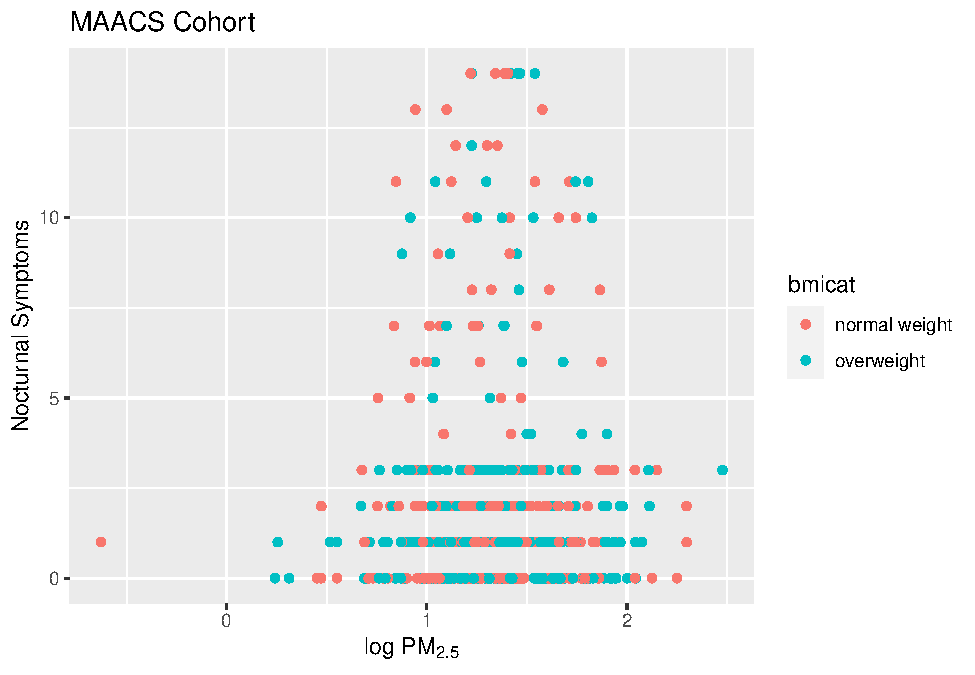
\includegraphics{semana_3_files/figure-latex/unnamed-chunk-29-1} \end{center}

\hypertarget{notas-y-futuras-lecturas}{%
\subsection{notas y futuras lecturas}\label{notas-y-futuras-lecturas}}

\begin{itemize}
\tightlist
\item
  \href{http://www-bcf.usc.edu/~gareth/ISL/}{Introduction to statistical
  learning}
\item
  \href{http://www-stat.stanford.edu/~tibs/ElemStatLearn/}{Elements of
  Statistical Learning}
\item
  \href{http://www.stat.washington.edu/raftery/Research/PDF/fraley2002.pdf}{Model
  based clustering}
\item
  \href{http://en.wikipedia.org/wiki/Linear_discriminant_analysis}{Linear
  Discriminant Analysis}
\item
  \href{http://en.wikipedia.org/wiki/Quadratic_classifier}{Quadratic
  Discriminant Analysis}
\end{itemize}

\end{document}
